%%%%%%%%%%%%%%%%%%%%%%%%%%%%%%%%%%%%%%%%%
% University Assignment Title Page 
% LaTeX Template
% Version 1.0 (27/12/12)
%
% This template has been downloaded from:
% http://www.LaTeXTemplates.com
%
% Original author:
% WikiBooks (http://en.wikibooks.org/wiki/LaTeX/Title_Creation)
%
% License:
% CC BY-NC-SA 3.0 (http://creativecommons.org/licenses/by-nc-sa/3.0/)
% 
% Instructions for using this template:
% This title page is capable of being compiled as is. This is not useful for 
% including it in another document. To do this, you have two options: 
%
% 1) Copy/paste everything between \begin{document} and \end{document} 
% starting at \begin{titlepage} and paste this into another LaTeX file where you 
% want your title page.
% OR
% 2) Remove everything outside the \begin{titlepage} and \end{titlepage} and 
% move this file to the same directory as the LaTeX file you wish to add it to. 
% Then add \input{./title_page_1.tex} to your LaTeX file where you want your
% title page.
%
%%%%%%%%%%%%%%%%%%%%%%%%%%%%%%%%%%%%%%%%%
%\title{Title page with logo}
%----------------------------------------------------------------------------------------
%	PACKAGES AND OTHER DOCUMENT CONFIGURATIONS
%----------------------------------------------------------------------------------------

\documentclass[12pt]{article}
\usepackage[english]{babel}
\usepackage[utf8x]{inputenc}
\usepackage{amsmath}
\usepackage{graphicx}
\usepackage[colorinlistoftodos]{todonotes}

\begin{document}

\begin{titlepage}

\newcommand{\HRule}{\rule{\linewidth}{0.5mm}} % Defines a new command for the horizontal lines, change thickness here

\center % Center everything on the page



\includegraphics{logo.png}\\[.1cm] % Include a department/university logo - this will require the graphicx package

%----------------------------------------------------------------------------------------
%	HEADING SECTIONS
%----------------------------------------------------------------------------------------

\text{\LARGE Department of Computer Science and Engineering}\\[1.5cm] % Name of your university/college

%
\textsc{\Large Report on }\\[0.5cm] % Major heading such as course name
%----------------------------------------------------------------------------------------
%	TITLE SECTION
%----------------------------------------------------------------------------------------

\HRule \\[0.4cm]
{ \huge \bfseries ARA – The Ant-Colony Based Routing Algorithm for MANETs}\\[0.4cm] % Title of your document
{Mesut G¨unes, Udo Sorges, Imed Bouazizi}
\HRule \\[1cm]
 
%----------------------------------------------------------------------------------------
%	AUTHOR SECTION
%----------------------------------------------------------------------------------------

\begin{minipage}{0.5\textwidth}
\begin{flushleft} \large
\emph{Report Writers:}\\
Shantanu Sarkar\newline(0416052041) \newline % Your name
Mahmud Ahmed\newline(0416052027) \newline
Md. Mostafizur Rahman\newline(0416052032) 
\end{flushleft}
\end{minipage}
~
\begin{minipage}{0.4\textwidth}
\begin{flushright} \large
\emph{Supervisor:} \\
Dr. Ashikur  Rahman% Supervisor's Name
\end{flushright}
\end{minipage}\\[1cm]



% If you don't want a supervisor, uncomment the two lines below and remove the section above
%\Large \emph{Author:}\\
%John \textsc{Smith}\\[3cm] % Your name

%----------------------------------------------------------------------------------------
%	DATE SECTION
%----------------------------------------------------------------------------------------

{\large \today}\\[.5cm] % Date, change the \today to a set date if you want to be precise

%----------------------------------------------------------------------------------------
%	LOGO SECTION
%----------------------------------------------------------------------------------------


 
%----------------------------------------------------------------------------------------

\vfill % Fill the rest of the page with whitespace

\end{titlepage}

\tableofcontents

\newpage
\begin{abstract}
Wireless adhoc network consists of set of nodes, having a fixed transmission range, which communicate among themselves through wireless medium in multi-hop manner. They nodes are practically hugely mobile which makes the process of route finding followed by data transmission more difficult in real life applications. Several algorithms have been proposed till now with their respective pros and cons over several performance aspects of wireless networks such as the transmission redundancy, reliability, overheads, delivery rates, etc. In this report, we introduced a new method, called Ant Colony Based Routing Algorithm, which is built upon the skillful problem solving capability of ants, inspired from swarm intelligence. This reports also includes elaborate simulations result which compare the performance of this newly introduced algorithm with existing other well-known algorithms names AODV, DSDV and DSR which shows this new algorithm more effective, scalable and efficient in various real life networks.
\end{abstract}

\section{Introduction}
A mobile ad-hoc network (MANET) is a flexible, infrastructure less set of mobile nodes communicating over radio in wireless medium. Each node has a fixed limited transmission range which causes the communication traffic to be relayed over several intermediate nodes lying in its transmission range. Hence, the name, “Mobile Multi-hop Ad-hoc Networks”, has been evolved from its nature of transmission. The primary goal or the prime obstacle in MANET is finding of a route between the communicating end-points. This problem becomes much severe when the mobility of the nodes is enhanced or increased.

In Figure \ref{adhoc}, we present a sample of a wireless adhoc network consisting 8 nodes marked AS \textit{A,B,C,D,E,F,G,H}. An edge is inserted between two nodes lying in each other transmission range. For example, node B is situated in the transmission range of A, so A and B are connected and this follows for the rest of nodes also.



This report sheds light on a new approach of path setting for communication between points in wireless mobile networks based on swarm intelligence. Swarm intelligence (SI), introduced by Gerardo Beni and Jing Wang in 1989, employed in work on artificial intelligence, is built on collective behavior of distributed systems, natural or artificial.  Examples in natural systems of SI include ant colonies, bird flocking, animal herding, bacterial growth, fish schooling and microbial intelligence. 


We will be using Ant Colony Algorithm, a sub-set from Swarm Intelligence, and  use the ability of simple ants to solve complex problems by cooperation without any direct communication, rather by stigmergy, to devise optimized routing algorithm in the scenario of mobile wireless adhoc networks. The essence of finding complete routing algorithm in the wireless adhoc network emergence from the importance of these kinds of networks. These type of networks are very much fragile which makes it highly adaptable in disaster and military applications, vehicular networks, Ubiquitous computing, Sensor Networks, etc. The newly presented on-demand routing algorithm based on ant colony based meta heuristics is highly adaptive, efficient and scalable because the performance remains almost the same irrespective of dense or sparse network, irrespective low or high mobility, etc. 

\begin{figure}
    \centering
    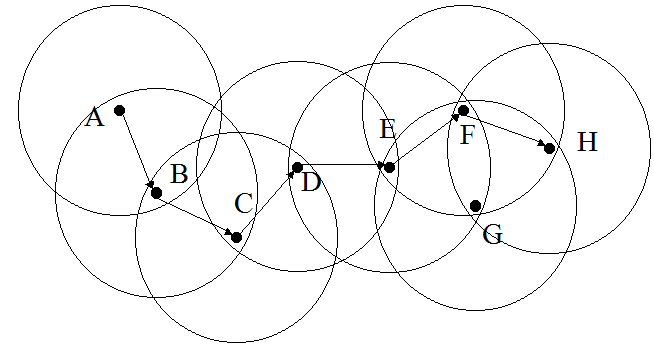
\includegraphics[scale=0.5]{adhoc}
    \caption{Wireless Adhoc Network}
    \label{adhoc}
\end{figure}

\section{Background studies}
The Ant-Colony-Based Routing Algorithm(ARA) used in this paper is a particular class of ant algorithms which is based on swarm intelligence. It is a multi-agent systems algorithm which consists of agents with the behavior of individual ants. It is found that in routing algorithms a lot of swarm intelligence based routing algorithm performs really well. The basic algorithms for ARA is really simple which is described in the later section.


\section{Methodology}

\subsection{Basic Ant Algorithm}

The basic ant algorithm is simulated on the food searching behavior of ants. Leaving from their home, ant searches for food tracing the smell or some other indicator of foods. Coming upon a diversion or an obstacle, it randomly chooses a path and starts going along that path. But interestingly, they leave some pheromone while they move on a specific path. So the amount of pheromone is used as an measure of number of ants going in a specific path. Obviously the shortest path from the nest up to the food location gradually has the higher amount of pheromone which helps the ants coming later on that diversion to choose the path. The ants choose the path which has the higher pheromone concentration in a distributive fashion throughout the entire path. With time being elapsed, the concentration of pheromone is diffused and thus decreased which makes the path searching process dynamic.

\begin{figure}
    \centering
    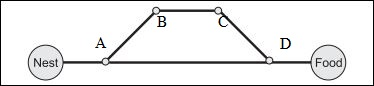
\includegraphics[scale=0.9]{ant2}
    \caption{Ant Colony Algorithm}
    \label{ant}
\end{figure}

In figure \ref{ant}, the above scenario is described. Coming to an intersection point A, a few ant goes through path AB and randomly some other ants follows the path AD towards the food. But the ants that going through the path AD will reach the food quite fast and thus the number of ants following this path will increase which in turns increases the amount of pheromone along this path. As a result, in the long run, when other ants will come to this intersection point, it will assess the amount of pheromone and find its concentration higher in the path AD and thus the shortest path will be converged. 

\subsection{Ant Colony Optimization Algorithm for Routing}
So, in accordance with such behavior of ant, when a data packet comes to a node, it chooses an outgoing edge from that node with a specific probability, calculated by dividing the amount of pheromone of that edge by the total amount of pheromone of all the outgoing edge from that node. When an edge has been chosen for data transmission, the amount of pheromone of that edge is increased by a fixed amount to mark that the edge is being used highly for data passing. The amount of pheromone is also decreased with time by a fixed amount to engage dynamicity. The equations are listed in figure \ref{eq}. The probabilty of picking an edge \textit{ij} is the amount of pheromone of edge \textit{ij} divided by the total pheromone value of all \textit{j} edges outgoing from \textit{i}, as described in \textit{equation 1}. Obviuously, the sum of the probabilty of choosing all the edges be 1, as we see in \textit{equation 2}. While an edge been chosen, it's concentration of pheormone is increased by $\delta \phi$ and with time, its concentration of pheromone is reduced by a certain amount, q, as listed in \textit{equation 3 and 4 }

\begin{figure}
    \centering
    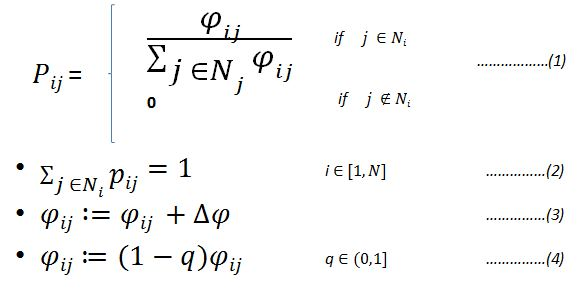
\includegraphics[scale=0.6]{equations}
    \caption{Equations for ACO}
    \label{eq}
\end{figure}

\subsection{The Routing Algorithm}

\subsubsection{Route Finding}
This phase is done using two type of data packets: FANTs used to track pheromone to source node and BANTs used to track pheromone to destination node. Being broad casted by the sender, A node receiving a FANT creates a record consisting destination address, next hop and
pheromone value in its routing table.. Thus being relayed upto he destination node, it extracts the information of the FANT,  destroys it and releases BANT in similar manner as of the FANTs to the source which sets up the path for data transmission.

In figure \ref{rfp}, we showed the process of route finding, starting from node S and as destination upto node D. The intermediate nodes are used to recieve the FANT packets and transmit to the destination and also to recieve the BANT packets and tranmit it to other direction. The green direction is the flow of FANT packets and the Orange one for the BANT packets.
\begin{figure}
    \centering
    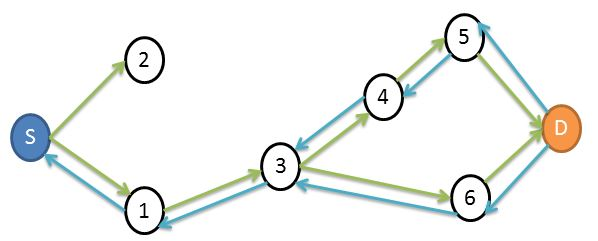
\includegraphics[scale=0.6]{fantbant}
    \caption{Route Finding Process}
    \label{rfp}
\end{figure}

\subsubsection{Route Maintenance}
The data packets are used to maintain the path by increasing the amount of pheromones of that edges through which they travel. Duplicate packets are identified through the unique sequence number and detecting the duplicates, the DUPLICATE ERROR flag and the packet is sent back to the previous node followed by the deactivation of that link. In figure \ref{duperr}, we show this process, where a same packet came from node 2 and 3. So setting DUPLICATE ERROR flag = 1, the path node 3 to 4 has been deactivated.

\begin{figure}
    \centering
    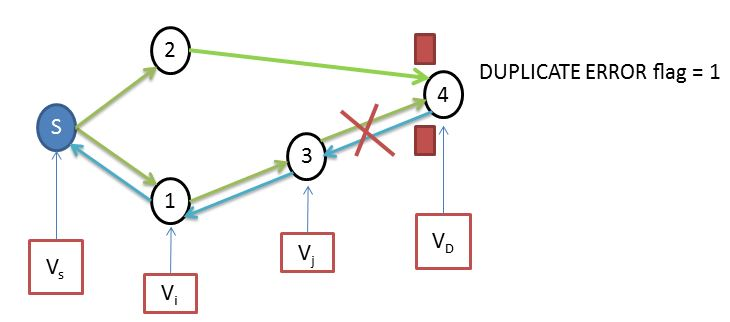
\includegraphics[scale=0.6]{duperr}
    \caption{Route Maintenance Process}
    \label{duperr}
\end{figure}


\subsubsection{Route Error}
Recognizing a route failure through a missing acknowledgement, a node, receiving ROUTE Error Messge, deactivates a link setting pheromone value of that link as 0. The it searches for an alternate link. If it finds then it sends the packet through that path, otherwise, it informs its neighbors. If the packet does not reach the destination, the source initiates a new route discovery phase.

\begin{figure}
    \centering
    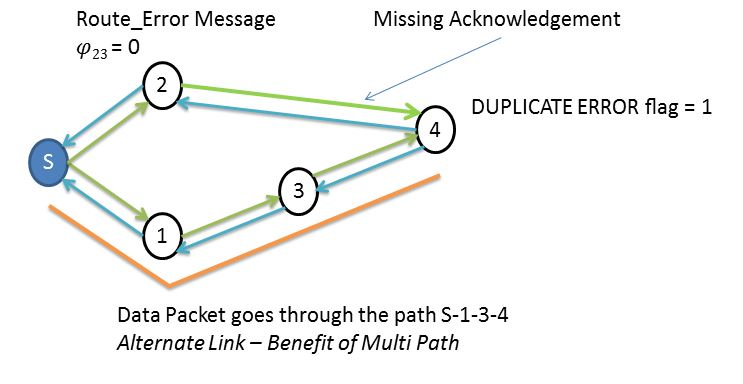
\includegraphics[scale=0.6]{rout}
    \caption{Route Error Process}
    \label{rout}
\end{figure}

This scenario has been depicted in figure \ref{rout}. Here, acknowledgement has been missing in the link of \textit{34}. So, setting the pheromone of this edge as 0, the packet goes in aother alternate path as shown in the figure. If this path was not there and the packet backtracked to the root, it would have to initiate another rout finding process. 

\subsection{Worthiness of ARA}

With a view to measuring the worthiness of presented algorithm, the authors jotted down the characteristics of their presented algorithm, calculated the overhead this algorithm and also confirmed their calculations by measuring the performance metrics like throughput, delivery rate, overheads in terms of packets and data bit, etc.

\subsubsection{Characteristics of ARA}
The authors picked the following reasons to prove the diligence of this algorithm. This reasons basically illustrates different aspects
why this kind of algorithms could perform well in mobile
multi-hop ad-hoc networks. 

\begin{itemize}
  \item Supports Dynamic topology
  \item being distributed algorithm
  \item Support for multi-path
  \item Chance for measuring link quality
  \item Prevents loop in the topology.
  \item Provides Demand-based operation
  \item Provides sleep mode operations.
\end{itemize}

\subsubsection{Overheads of ARA}
The authors measured the overhead of this algorithm which is very small, because of no interchange of routing tables between the nodes. Unlike other routing algorithms like DSDV or DSR, it doesn't exchange routing table information, which restricts ARA's overhead to minimal stage. Just a unique sequence number is transmitted in the routing packets to prevent the duplicated packets. Even  no extra packets are needed for route maintenance, the data packets only carries the IP header, for which there is no extra burden of overhead.


\textbf{Remark.} The authors also confirmed the worthiness of their solution by calculating the throughput, delivery rate of the packets and the overhead in terms of packets and data bits.


\section{Evaluation Metrics}
According to the Authors, the main feature of ARA is its low routing overhead and easy maintainability of routes between nodes in the topology. So, The evaluation metrics considered to measure the performance of ARA are:
\begin{itemize}
\item Delivery rate 
\item Routing overhead in terms of bits
\item Routing overhead in terms of packets
\end{itemize}

\section{Evaluation Process}\label{simulationenv}
The performance of ARA was evaluated using simulation in terms of evaluation metrics mentioned earlier. 
The simulation was implemented in ns-2. Some important parameters of the simulation environment are:

\begin{itemize}
\item Simulation area  1500m×300m 
\item Maximum velocity of nodes 10 m/s using Random waypoint model.
\item Simulation time  900 seconds
\item 10 Constant bit rate(CBR) connections
\item 7 different pause times\footnote{pause time indicates the mobility of the nodes} 0,30, 60, 120, 300, 600 and 900 seconds
\end{itemize}


\section{Evaluation Results}
Multiple simulations were run and the results were collected for evaluation. 
\subsection{Comparison with existing routing protocols in delivery rate}
The best way to evaluate the performance of a new algorithm is to compare the performance with the existing algorithms. So, the performance of ARA was compared with AODV,DSR and DSDV in terms of delivery rate. The observed results are shown in Figure~\ref{fig:picture1}. With high mobility both DSR and ARA has more than 95\% delivery rate. 
Throughout the simulations ARA performed better than DSDV and AODV in this criteria. Figure~\ref{fig:picture2} shows the delivery rate of ARA within the confidence interval of 95\%. As we can see All results are above 85\% and most results are within the range 90\% and 100\% throughout the 10 simulation runs.


\begin{figure}[t!]
\centering
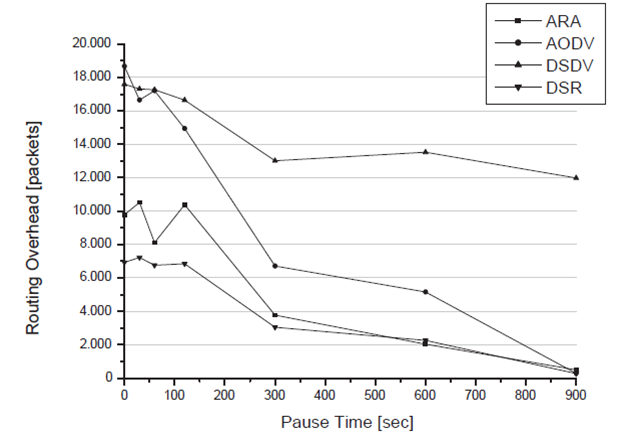
\includegraphics[width=0.7\textwidth]{Picture1.png}
\caption{\label{fig:picture1}Successful delivered packets as a
function of pause time.}
\end{figure}


\begin{figure}[t!]
\centering
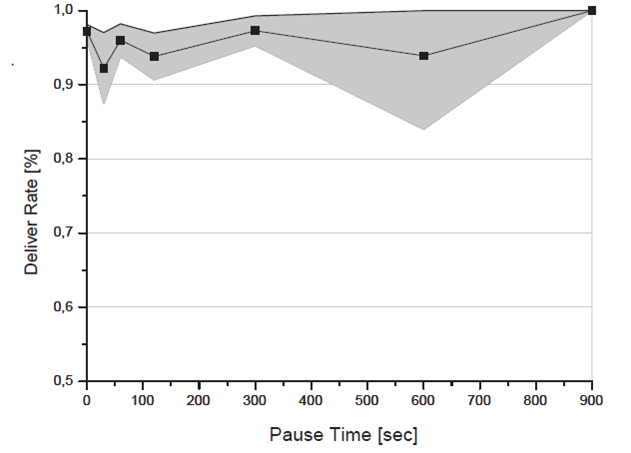
\includegraphics[width=0.7\textwidth]{Picture2.png}
\caption{\label{fig:picture2}Delivery rate of ARA. Confidence interval of 95\%}
\end{figure}


\subsection{Routing Overhead Comparison}
As different protocols generate the overhead in very different ways, the routing overhead of different algorithms were observed both in terms of fraction of routing packets needed to deliver a data packet and fraction of databits needed for routing.
\subsubsection{Routing Overhead in terms of databits}
Figure ~\ref{fig:picture3} shows the routing overhead of routing algorithms in term of routing bit as a fraction of total databits. In this case ARA give the best results throughout the simulations. Figure ~\ref{fig:picture4} show the overhead of ARA in 95\% confidence interval.
  
\begin{figure}[t!]
\centering
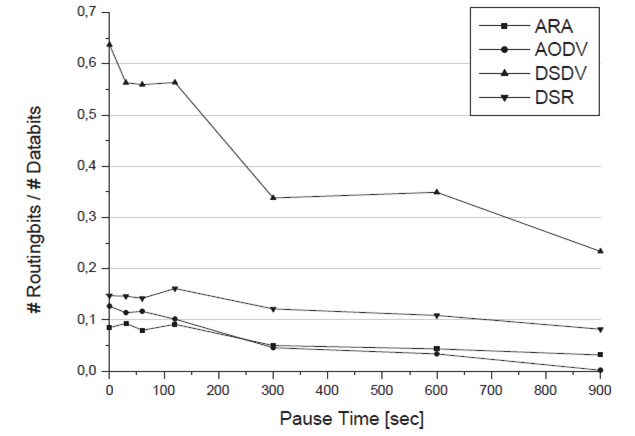
\includegraphics[width=0.7\textwidth]{Picture3.png}
\caption{\label{fig:picture3}Pause time vs Fraction of successfully send bits and the needed bits}
\end{figure}

\begin{figure}[t!]
\centering
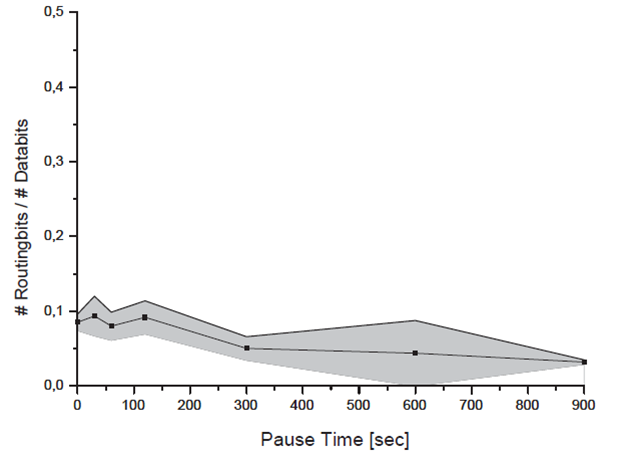
\includegraphics[width=0.7\textwidth]{Picture4.png}
\caption{\label{fig:picture4}Overhead of ARA in bits. Confidence interval of 95\%}
\end{figure}



\subsubsection{Routing Overhead in terms of packets}
Figure ~\ref{fig:picture5} shows the routing overhead of routing algorithms in term of packets. In this case ARA give second best results following DSR.This is due to the needed flooding of the approach in the route finding phase. With high node mobility route failure occur more often, thus requires the
performing of the route failure handling part of the algorithm,which in worst case has to backtrack the path until
the sender. Figure ~\ref{fig:picture6} show the overhead of ARA in 95\% confidence interval.
  
\begin{figure}[t!]
\centering
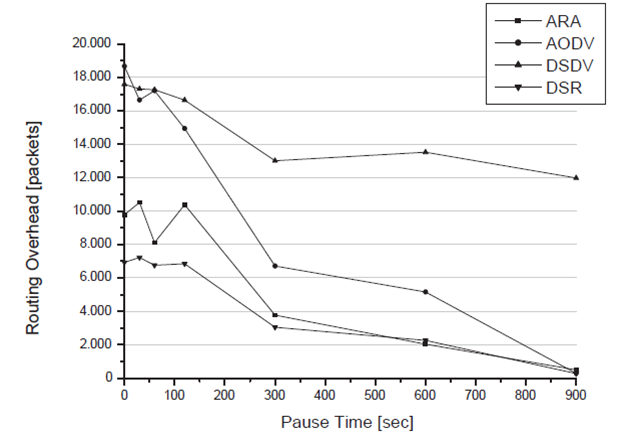
\includegraphics[width=0.7\textwidth]{Picture5.png}
\caption{\label{fig:picture5}Pause time vs Fraction of successfully send bits and the needed bits}
\end{figure}

\begin{figure}[t!]
\centering
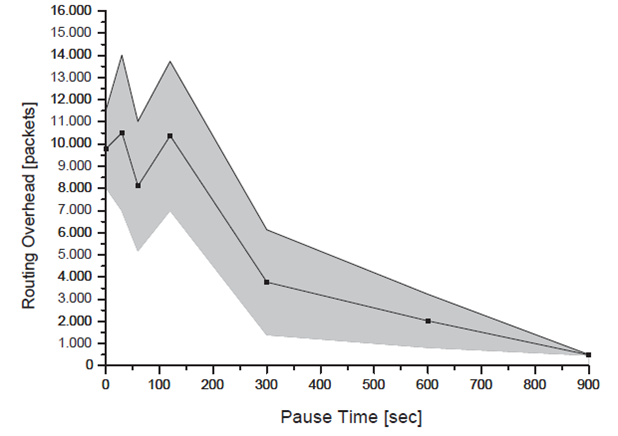
\includegraphics[width=0.7\textwidth]{Picture6.png}
\caption{\label{fig:picture6}Overhead of ARA in packets. Confidence interval of 95\%}
\end{figure}


\textbf{Remarks:}The authors used standard simulation processes to collect data under the simulation environment in Section~\ref{simulationenv}. So, the collected data are reliable and trustworthy. ARA is a good choice for mobile networks in terms of data delivery,routing overhead. But a better conclusion can be derived if individual performances of DSR,DSDV,AODV were presented in 95\% confidence interval like Figure ~\ref{fig:picture2}, Figure ~\ref{fig:picture4}, Figure ~\ref{fig:picture6}. In that case we would be able to observe the fluctuations of performance over different mobility. 
Nevertheless, we consider ARA as a robust and highly maintainable routing protocols in mobile adhoc networks. 

\section{Limitations of ARA}
In this paper the routing algorithm implemented for mobile multi-hop wireless ad-hoc networks for a dynamic topology works closer to DSR but with a lesser overhead. But routing problem still remains the main challenge for mobile multi-hop wireless ad-hoc networks. In this algorithm there are other aspects that could be evaluated. For instance we  could introduce a difference topology for a different kind of dynamic environment. In more dynamic environment this algorithm performs worse than DSR. In those kinds of environment we could calculate the pheromone in a different way that might give us better result by trial and error. Though this algotithm works better but it does not fit best for all kinds of application. High network load and multimedia data are the fields that are still needed to be evaluated. Maintenance of pheromone is also a crucial part for this algorithm which can be improved to give better perrformance.

\section{Future Works}
\begin{itemize}

\item Maintenance of pheromone concentration is the most crucial part of this algorithm. Pheromone concentration can be calculated differently for different kinds of dynamic environment which may give better performance for certain scenerio. High network load and multimedia data are fields that can be extended for this algorithm. Since node mobility is the main factor for mobile multi-hop wireless ad-hoc networks if we could predict the mobilty for a certain environment and set the pheromone concentration accordingly of a node that might result in a improved performance.

\item This algorithm was designed for mobile multi-hop wireless ad-hoc networks. So we can actually apply it to VANET by tweaking it to work with highly mobile network. Though it may have worse performance since this algorithm is designed particularly for MANET. If we we consider the mobility of a vehicle and if the mobility is not very high than this algorithm might give an average output.
\end{itemize}

\section{Conclusion}
The proposed ARA-Ant colony based rouging algorithm provides some great insights in mobile ad hoc networks.The approach is based on swarm intelligence and especially on the ant colony optimization meta-heuristic. The easy maintainability and low routing overhead of ARA gives better utilization of resources in the networks than other algorithms. Although there are some drawbacks of ARA and there are many scopes of improvements, we believe ARA is a good candidate for mobile ad hoc networks.





\newpage
\begin{thebibliography}{9}
\bibitem{latexcompanion} 
E. Bonabeau, M. Dorigo, and G. Theraulaz. Swarm intelligence:
from natural to artificial intelligence. Oxford University
Press, 1999. ISBN 0-19-513158-4.
 
\bibitem{einstein} 
J. Broch, D. A. Maltz, D. B. Johnson, Y.-C. Hu, and
J. Jetcheva. A performance comparison of multihop wireless
ad hoc network routing protocols. Proceedings of the
Fourth Annual ACM/IEEE International Conference on Mobile
Computing and Networking (MobiCom’98), pages 85–
97, 1998.
 
\bibitem{knuthwebsite} 
M. Dorigo and G. Di Caro. The ant colony optimization
meta-heuristic. In D. Corne, M. Dorigo, and F. Glover, editors,
New Ideas in Optimization, pages 11–32. McGraw-
Hill, London, 1999.

\bibitem{}
C. E. P. (Editor). Ad Hoc Networking. Addison-Wesley,
2001. ISBN 0-201-30976-9.

\bibitem{}
K. Fall and K. Varadhan. The ns Manual, Nov 2000.

\bibitem{}
D. B. Johnson, D. A. Maltz, Y.-C. Hu, and J. G. Jetcheva.
The dynamic source routing protocol for mobile ad hoc
networks. IETF Internet draft, draft-ietf-manet-dsr-04.txt,
November 2000.
\bibitem{}
J. P. Macker and M. S. Corson. Mobile ad hoc networking
and the IETF. Mobile Computing and Communications
Review, 2(1):9–14, 1998.
\bibitem{}
C. E. Perkins and P. Bhagvat. Hihgly dynamic destinationsequenced
distnace-vector routing (dsdv) for mobile computers.
Computer Communications Rev., pages 234–244,
October 1994.
\bibitem{}
C. E. Perkins, E. M. Royer, and S. R. Das. Ad hoc ondemand
distance vector (aodv) routing. IETF Internet draft,
draft-ietf-manet-aodv-07.txt, November 2000.
\end{thebibliography}





\end{document}